En komparator tar inn et signal og sammenligner det med en referansespenning.

\begin{circuitikz} \draw
(4.5,4.5) node[op amp] (opamp) {}
(opamp.+) node[left] {signal}
(opamp.-) node[left] {ref}
(opamp.out) node[right] {ut}
      ;
\end{circuitikz}

Den gir utslag (0 eller 1) når signalet overstiger referansen.

\begin{figure}[H]
  \centering
  \caption{Komparator indikerer overstigelse av referanse}
  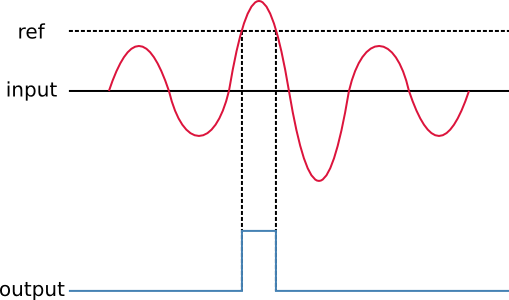
\includegraphics[width=0.67\textwidth]{./img/komparator}
\end{figure}
